

\section{Overview}
The team began by gathering requirements and deriving a system design, while creating a risk register in parallel. Where necessary, informal specifications were written to allow teams to develop components in parallel. The team individually tested their components throughout development. Once all components were completed they were integrated together, and the team assessed whether the system met their requirements.

\section{Requirements Analysis} \label{requirements}

Some general requirements have been made directly from the initial brief (marked as B below), which were then extended to include those that our prototype solution requires (marked as P). The aim was to show as many elements of our final solution as possible. Due to the cost and time it would take to prototype a satellite, this was left out of the prototype goals. Each other element in the system will be demonstrated to some level of implementation as this was achievable within the timeframe, budget and skills of the team. 

An evaluation of which requirements were implemented was done at each weekly meeting to ensure timely progress and allowed the group to focus on the requirements that had not yet been implemented rather than adding extra functionality. 
    
\textbf{Hardware}
\begin{enumerate}
\item There must be a demonstration of a locking mechanism (P)
\item The locking mechanism must unlock with only one key (P)
\end{enumerate}

\textbf{Backend}
\begin{enumerate}[resume]
\item There must be a connection to a Redis database from the application (P)
\item Route planning must be implemented (B)
\item Constraints must be incorporated within the final route plan (P)
\end{enumerate}

\textbf{Courier View}
\begin{enumerate}[resume]
\item There must be step-by-step guidance from the origin to the destination (B)
\item There must be a way to communicate with the control room (P)
\end{enumerate}

\textbf{Customer View}
\begin{enumerate}[resume]
\item The customer must be able to see the ETA of the package (P)
\item The customer must be able to see the current status of the delivery (P)
\end{enumerate}

\textbf{Control Room View}
\begin{enumerate}[resume]

\item The supervisor must be able to view all couriers (P)
\item The supervisor must be able to view all customers (P)
\item The supervisor must be able to view all deliveries (P)
\item The supervisor must be able to view a map showing all couriers (P)
\item The supervisor must be able to add couriers/customers/deliveries (P)
\item The supervisor must be able to add constraints to everyone/customers/deliveries (P)
\item The supervisor must be able to communicate with the courier

\end{enumerate}

Requirements 1 and 2 were generated due to the reasoning in Section \ref{databasearch}. The need for requirement 3 comes from the importance of storing the information used throughout the rest of the application - information regarding customers, deliveries, couriers, messages and constraints are all stored here. Redis was the database of choice due to its enhanced security features detailed in Section \ref{databasearch} and as it is easy to setup. Requirements 4 and 6 came directly from the original brief detailing the need of a "routing system capable of guiding a courier “step by step”. 

Requirements 5 and 15 come from the system being mission-critical which means it is essential for the package to reach its final destination. The ability to constrain the route enables both the customer and the controller to tell the routing system to avoid certain areas and also ensure the destination is reached in time. Requirements 7 and 16 ensure that the courier has up to date information regarding the routing and also means any specific information can be sent in text for clarification. The courier can also let the control room know of any possible routing implications that have not been picked up by the mapping API or whether they are in any imminent danger. 

Requirements 8 and 9 are necessary as this is what the customer will see and enables the demonstration to show all aspects of the application.

Requirements 10-13 allow the supervisor in the control room to have a full overview of the system and which deliveries are active and how they are all progressing. Requirement 14 means they can add new information in to the frontend which will then update the Redis database. This allows all supervisors to have the same information displayed to them and again, allows full control. If this system was taken forwards and brought to market, it may be worthwhile implementing different levels of access for supervisors as they may eventually have different roles to each other. E.g. maybe some supervisors are responsible for verifying routes/managing risks where as some have a more administrative role of adding couriers/deliveries.




\section{Design}

After collecting the requirements for the system we created a basic block diagram of the components of the system that we would like to created. A subset of these components have then been implemented in the prototype of the system. This diagram can be seen in \ref{fig:SystemDesign}. It is worth noting that under normal operation the only communication that goes over the internet is to the customer who gets only a limited view of the data. 

\begin{figure}[h]
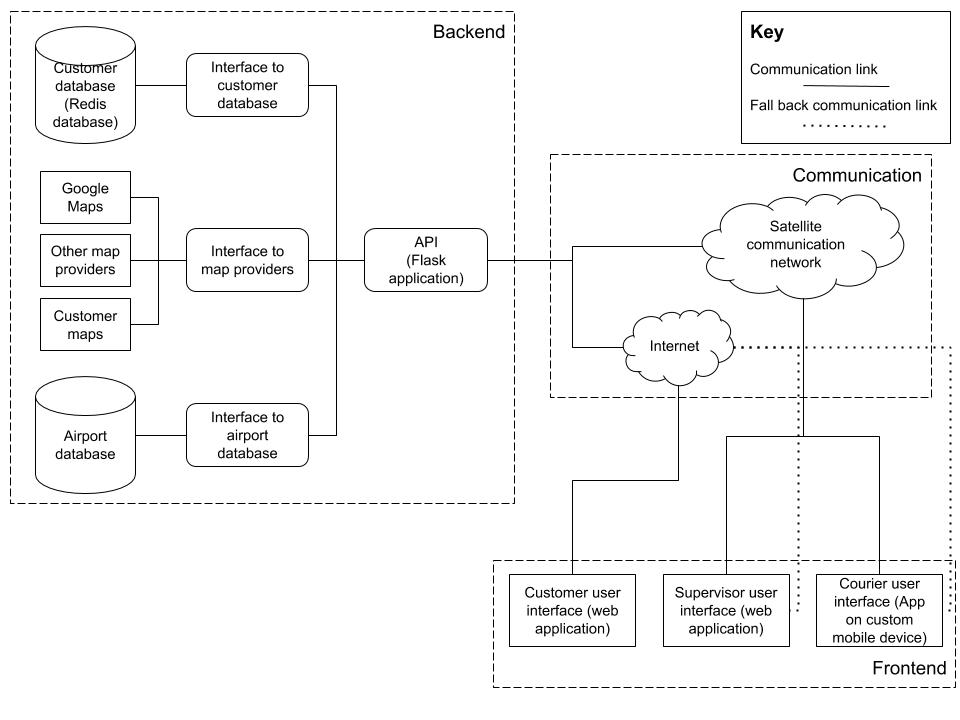
\includegraphics[scale=0.5]{SystemDesign.jpg}
    \centering
    \caption{Diagram of the overall system design}
    \label{fig:SystemDesign}
\end{figure}

As part of designing the final solution, a risk assessment was performed. This enabled the team to develop our initial ideas into something more concrete, ensuring major risks to the whole system including the courier, briefcase and communication were taken in to account, as when combined, securing these parts of the system ensures that the packages reach their final destination. The risk assessment findings were documented in a risk register table as seen in Table \ref{tab:riskRegister}.

The risk register scores each risks based on two factors - Impact (I) and Likelihood (L) to give an overall score of Severity (S). Each risk is given an ID which contains a unique number and what the risk applies to/comes from. The categories are as follows: Communication/Transport (C), Briefcase (B), Courier  (M) or General (G). Each of these is rated on a scale of 1 to 5 where 5 is very likely/has a high impact/is very severe. Each risk has a risk status which can either be Identified (I), Controlled/Accepted (C) or Resolved (R). The risks to the project itself are shown within Appendix \ref{tab:projectrisks}, these were considered to ensure completion of the prototype, report and presentation to a high standard.


\newcommand{\specialcell}[2][c]{%
  \begin{tabular}[#1]{@{}p{0.5\textwidth}@{}}#2\end{tabular}}
  

\begin{longtable}{|p{0.05\textwidth}|m{0.27\textwidth}|p{0.5\textwidth}|p{0.08\textwidth}|}

\hline
    \textbf{ID} & \textbf{Risk Description} & \textbf{Mitigation (M) and/or Contingency (C) Actions} & \textbf{Risk Status} \\
\hline
1-M & Courier becomes too ill to be able to carry out the transportation of the secured item
I-5 L-2 S-4 & \specialcell{M: Ensure that the courier is in good health before being sent out on a delivery \\
C: Both the courier’s and the briefcase’s location will be tracked throughout and a replacement courier will be sent to continue with the delivery} & C \\
\hline
2-M & Courier would like to steal the contents of the briefcase
I-5 L-2 S-4 & \specialcell{M: The courier will be subject to extensive background checks prior to being hired to carry out specific projects.\\
M: The briefcase will have a secure mechanism that only the recipient of the data can unlock \\
C: The item self destruct (along with approval from the customer) if a wrong key is entered in to the lock} & C \\
\hline
3-M & Courier is maliciously intercepted whilst en route
I-4 L-1 S-3 & \specialcell{M: The courier will not be sent through high-risk countries/areas, according to a continuously updated database which provides constraints for the courier\\
M: The courier will not advertise that they are carrying a high security item\\
M: There will be many dummy map requests in addition to the one actually used by the courier making it harder to find the true location from the outside \\
C: There is a panic button on both the briefcase and the navigation device that the courier can use to alert the control room to any issues} & C \\
\hline
4-M & Vehicle the courier is using breaks down
I-5 L-2 S-4 & M: Ensure a reliable firm is used for hiring cars and that the cars have been recently serviced
C: The vehicles used by the couriers will have specialist insurance to cover them through the countries they will be visiting & C \\
\hline
X-Y & Transferred to fake courier & M: The new courier will have to plug in their uniquely identifiable USB to complete the transfer and prove it is them. They will also carry photo identification so this will mean multi-factor authentication will be used to transfer the briefcase & C \\
\hline
5-G & Project goes over budget
I-? L-? S-? & M: Ensure thorough planning and include an unexpected costs section in case of emergencies & I \\
\hline
6-C & Communication satellite goes down meaning that the control room cannot contact or send updates to the courier
I-4 L-1 S-3 & \specialcell{M: The courier will download their route so they can access it offline if needed\\
M: Multiple satellites will be launched at once in case one fails} & C \\
\hline
7-C & Map functionality is not up to date
I-3 L-3 S-3 & M: Ensure the most frequently updated mapping tools are used & I/C \\
\hline
X-C & Parameter Overwrite Injection & M: Commands to the Redis database would be renamed within the code and therefore the attackers would not know the name of the functions to call in order to access the database & C \\
\hline
8-B & There is a risk that the electronic locking mechanism fails
I-5 L-3 S-4 & \specialcell{M: Thorough testing of the device will be carried out prior to the product being created for use in the field\\
C: Self destruct could also be activated if the locking mechanism fails and this choice has been made by the customer} & I/C\\
\hline
9-B & Battery for the electronic locking mechanism runs out
I-5 L-3 S-4 & \specialcell{M: Ensure the original battery has enough capacity to fulfil one delivery\\
M: The locking mechanism defaults to locked when out of power\\
C: Ensure the courier is carrying a spare battery\\
C: The briefcase will have a USB port enabling the battery to be charged} & R \\
\hline
 \caption{Risk Register}
    \label{tab:riskRegister}
\end{longtable}

Additionally to the risk register, members of the group wrote a simple outline of the customer database, and used this to derive a specification of the API. Other members of the team researched the Google Maps API and developed a specification for the routes section of the API in parallel. All the external tools used in the product (Redis, Google Maps, Docker) were discussed in meetings, and the team decided which were suitable for the product in terms of functionality, security, and personal experience. All design documents produced were reviewed by all members of the team prior to being used in development.

\section{Development}

These specifications allowed frontend and backend development to progress in parallel over 5 weeks, along with the briefcase prototype. Development began on the 30th of April and completed on the 3rd of June. Prior to integration, the team was distributed as follows:

\begin{itemize}
    \item Frontend: 3 developers
    \item Backend: 2 developers
    \item Briefcase: 1 developer
\end{itemize}

The frontend team developed the supervisor and courier components based on the specification of what functionality the backend would provide, while the backend team programmed their solution to deliver this functionality as specified. In a few cases, the backend team decided to deviate from the specification to deliver the same functionality in a simpler manner, or the frontend team requested slighttly different features. Whenever changes were necessary this was communicated in meetings and over Slack, and the documentation was updated accordingly. Components were developed and tested on their own Git branches and merged after a thorough code review.

The entire team spent the final two weeks of development integrating the backend and frontend. Some wrote code, while others investigated and fixed bugs discovered throughout the process. Team members who had no tasks to complete at a given time compiled documentation for the report and presentation.

\section{Testing}
Due to the limited time available, the team did not impose any overall testing standards for the project. Members tested their components as they felt necessary. The frontend underwent a user acceptance test using a web browser. The routing API was manually tested using the Insomnia REST client. We decided against unit testing due to the variability of routes, as it would be impossible to achieve thorough coverage. Additionally, this component relies on Google Maps, which we trust has been thoroughly tested, though we aim to test it was integrated correctly prior to a full product release. The database API was tested manually using Postman, and unit tested to complete functional coverage. This component was tested more thoroughly due to the frontend relying heavily on it.

These tests allowed us to develop a working prototype. However, our product is mission critical, and as such requires thorough automated testing of every component to a higher standard of coverage prior to deployment.
